% This is LLNCS.DEM the demonstration file of
% the LaTeX macro package from Springer-Verlag
% for Lecture Notes in Computer Science,
% version 2.4 for LaTeX2e as of 16. April 2010
%
\documentclass{llncs}
%
\usepackage{makeidx}  % allows for indexgeneration
\usepackage{url}
\usepackage[inline]{enumitem}
\usepackage{todonotes}
\usepackage{hyperref}
\usepackage{todonotes}
\usepackage{subcaption}
\usepackage{multirow}

%
\begin{document}

\title{Geographical trends in research: \\a preliminary analysis on authors' affiliations}

\author{Andrea Mannocci, Francesco Osborne, Enrico Motta}
\authorrunning{Andrea Mannocci et al.} % abbreviated author list (for running head)
\institute{Knowledge Media Institute, The Open University, Milton Keynes, UK
\email{name.surname@open.ac.uk}}

\maketitle  % typeset the title of the contribution
\begin{abstract}
In the last decade, research literature reached an enormous volume with an unprecedented current annual increase of 1.5 million new publications. 
As research gets ever more global and new countries and institutions, either from academia or corporate environment, start to contribute with their share, it is important to monitor this complex scenario and understand its dynamics.

We present a study on a conference proceedings dataset extracted from Springer Nature Scigraph that illustrates insightful geographical trends and highlights the unbalanced growth of competitive research institutions worldwide.
Results emerged from our micro and macro analysis show that the distributions among countries of institutions and papers follow a power law, and thus very few countries keep producing most of the papers accepted by high-tier conferences.
In addition, we found that the annual and overall turnover rate of the top 5, 10 and 25 countries is extremely low, suggesting a very static landscape in which new entries struggle to emerge. 
Finally, we highlight the presence of an increasing gap between the number of institutions initiating and overseeing research endeavours (i.e. first and last authors' affiliations) and the total number of institutions participating in research.
As a consequence of our analysis, the paper also discusses our experience in working with affiliations: an utterly simple matter at first glance, that is instead revealed to be a complex research and technical challenge yet far from being solved.
\keywords{Scholarly knowledge, affiliations, conferences, scientometrics, research, scigraph}
\end{abstract}


%
\section{Introduction}
Over the last decade, research started to scale up in terms of produced volume of papers, authors and contributing institutions. 
Nowadays, research literature is estimated to round up 100-150 million publications with an annual increase rate around 1.5 million new publications~\cite{Bornmann2015}.
Such a complex, global-scale system is worth studying in order to understand its dynamics and internal equilibria.
In particular, the study of authors' affiliations~\cite{frenken2009,pan2012} has concrete impact on the interpretation of research as a complex phenomenon inserted in a delicate socioeconomic and geopolitical scenario.

In this study, we present an analysis on a dataset of conference proceedings metadata covering the 1996-2017 period, which was distilled from SciGraph\footnote{Springer Nature SciGraph, \url{https://www.springernature.com/gp/researchers/scigraph}}, a free linked open data (LOD) dataset about scholarly knowledge published and curated by Springer Nature.
%This dataset focuses on papers published in conference proceedings across several scientific disciplines such as computer science, life sciences, chemistry and engineering.
In particular, we first present a \textit{macro analysis} on the full dataset, including conference proceedings across several scientific disciplines (e.g. computer science, life sciences, chemistry, engineering) and then a \textit{micro analysis}, which focuses on three high-tier conferences close to our area of expertise: the International Semantic Web Conference (ISWC), the Extended Semantic Web Conference (ESWC), and the International Conference on Theory and Practice of Digital Libraries (TPDL).

The main contribution of this work is threefold.
Firstly, we found that, over the observed period, the distributions of institutions and papers among countries follow a power law, consistently to what previously demonstrated in the literature across the 1981-2010 period~\cite{may1997,king2004a,egghe2005power,pan2012}. 
Therefore, very few subjects keep producing most of the papers accepted by scientific conferences.
Secondly, we show how the annual and overall turnover rate of the top 5, 10 and 25 countries is extremely low, suggesting a very static landscape in which new entries struggle to emerge.
Finally, we highlight an increasing gap between the number of institutions initiating and overseeing research endeavours (i.e. first and last authors' affiliations) and the total number of institutions participating in research. 

% The remainder of this paper is structured as follows: in Section~\ref{sec:sota} we summarise the relevant state of the art. In Section~\ref{sec:data} we describe the criteria that drove us in the selection of the dataset, while in Section~\ref{sec:method} we describe the methodology for our analysis.
% Finally, in Section~\ref{sec:results} we describe emerged in our analysis and we summarise and conclude in Section~\ref{sec:discussion}.
% Finally, in Section~\ref{sec:conclusions} we recap and conclude.


\section{Literature Review}
\label{sec:sota}
A variety of bibliometrics studies in the last 30 years highlighted the importance of different factors (or \textit{proxies}) of the presumed quality of research produced by researchers, institutions, and countries. 
In particular, they showed how researchers' performance can be affected by factors such as gender~\cite{Jadidi2017}, location~\cite{frenken2009}, reputation~\cite{petersen2014reputation}, centrality in the co-authorship network~\cite{sarigol2014predicting}, online presence~\cite{thelwall2013altmetrics}, and so on. 
For instance, Jadidi et al.~\cite{Jadidi2017} investigated gender-specific differences on about 1 million computer scientists over the course of 47 years and observed that women are on average less likely to adopt the collaboration patterns associated with a strong research impact. Petersen et al.~\cite{petersen2014reputation} introduced an approach for quantifying the influence of an author reputation on their future research impact and found that reputation is associated with the citation count of articles, but only during the early phase of the citation lifecycle. Sarigol et al.~\cite{sarigol2014predicting} demonstrated that a classifier based only on co-authorship network centrality metrics can predict with high precision whether an article will be highly cited within five years after the publication. Thelwall et al.~\cite{thelwall2013altmetrics} showed that there is a significant association between eleven tested altmetrics and citations in the Web of Science dataset.

Some groundbreaking work focused in particular on the role of countries, cities, and organisations (e.g. university, research institutes) and highlighted the great discrepancy in quality and quality of the research produced by different nations. For instance, May~\cite{may1997} analysed the numbers of publications and citations of different countries in the 1981-1994 period using the Institute for Scientific Information database (Ed. then Thomson ISI and finally Clarivate Analytics), which included more than 8,4 million papers and 72 million citations. 
In accordance with our results, the authors found that the countries that produced the highest share of research papers more than 20 years ago were USA, United Kingdom, Japan, Germany, France, Canada, Italy, India, Australia, and Netherlands. King~\cite{king2004a} built on this work and analysed the 1993-2002 period adopting again the Thomson ISI dataset. 
Ten years after May's study, the most important countries regarding research were essentially the same.
In particular, King found that the countries that produced most of the top 1\% highly cited publications were USA, United Kingdom, Germany, Japan, France, Canada, Italy, Switzerland, Netherlands, and Australia. Pan et al.~\cite{pan2012} continued this line of work by performing a systematic analysis of citation networks between cities and countries in the 2003-2010 period. 
In accordance to our findings, they found that the citation distribution of countries and cities follows a power law.
According to their citation rank, the main producer of research in the period under analysis were USA, United Kingdom, Germany, Japan, France, Canada, China, Italy, Netherlands, and Australia.
Interestingly, they also argued that a necessary (but not sufficient) condition for a country to reach an impact larger than the world average is to invest more than about 100,000 USD per researcher annually.

Other studies are more restricted in scope and focus either on specific locations~\cite{carvalho2006,borner2005spatio,monroe2016inequalities} or on specific research areas, such as tropical medicine ~\cite{falagas2006bibliometric}, nanomedicine~\cite{woodson2012research}, biomedicine~\cite{falagas2006bibliometric2}, and e-learning~\cite{hung2012trends}. 
A good review of bibliometrics studies that explicitly take into account the spatial factor can be found in Frenken et al.~\cite{frenken2009}.
Unlike the aforementioned analyses, in this preliminary study we 
\begin{enumerate*}[label=(\roman*)]
\item focused on the temporal evolution of countries and institutions in conference papers,
\item performed an analysis on the first and last authors' affiliations, and
\item addressed specific high-tier conferences in the domain of semantic web and digital libraries during the 2003-2017 period.
\end{enumerate*}


\section{Data}
\label{sec:data}
A main premise for our study is the availability of a scholarly knowledge dataset containing information about authors' affiliations sufficiently detailed and structured, i.e. including both institution name and country, possibly disambiguated through a persistent identifier.

For the time being, given the preliminary character of this analysis, we kept intentionally out of consideration pay-walled data sources such as Scopus\footnote{Scopus, \url{https://www.scopus.com}}, Web of Science\footnote{Web of Science, \url{https://clarivate.com/products/web-of-science}}, and Microsoft Academic\footnote{Microsoft Academic, \url{https://academic.microsoft.com}}, and we focused on what can be freely retrieved on the Web, in the spirit of open and reproducible science~\cite{wilkinson2016fair}.

Some top-quality scholarly datasets such as DBLP~\cite{ley2009} and Semantic Scholar\footnote{Semantic Scholar, \url{https://www.semanticscholar.org}} are not apt to our study as they miss essential information about authors' affiliations.
Other datasets technically provide authors' affiliations, but the relevant metadata are often incomplete.
%Other datasets provide authors' affiliations with best-effort details. 
For example, Crossref\footnote{Crossref, \url{https://www.crossref.org}}, despite declaring a field devised for affiliations in their metadata API JSON format\footnote{ \url{https://github.com/Crossref/rest-api-doc/blob/master/api_format.md}}, provides in a minority of cases a simple array of affiliation strings.
Besides, affiliation strings often exhibit several well-known ambiguity issues due to
\begin{enumerate*}[label=(\roman*)]
\item alternate forms (e.g., ``Open University'' and ``The Open University''),
\item different languages (e.g., ``Universit\`{a} di Pisa'' and ``University of Pisa''),
\item different granularity and missing information (e.g., ``Knowledge Media Institute, Milton Keynes'').
\end{enumerate*}

After an analysis of current solutions for selecting a dataset curated at the source with regards to these aspects, our choice fell onto SciGraph\footnote{SciGraph datasets, \url{http://scigraph.springernature.com/explorer/downloads/}}, a LOD dataset published and curated by Springer Nature.
To the best of our knowledge, SciGraph is the only large-scale dataset providing reconciliation of authors' affiliations by disambiguating and linking them to an external authoritative datasets in terms of institutions (in this case GRID, the Global Research Identifier Database\footnote{GRID, \url{https://www.grid.ac}}).
In its entirety, SciGraph consists of 78 distinct datasets and includes about 2 billion triples describing research literature objects such as journal articles, conference papers, books, and monographs published by Springer Nature and spanning over a broad set of topics such as computer science, medicine, life sciences, chemistry, engineering, astronomy, and more.

For our analysis we focused on conferences proceedings as conferences are the focal point of networking and knowledge exchange among practitioners.
To this end, we downloaded from SciGraph the \textit{books} and \textit{book chapters} datasets spanning from 1996 to 2017 and the \textit{conferences} dataset linking together all the books related to the same conference series.
Additionally, we downloaded the ancillary GRID dataset\footnote{GRID dataset, \url{https://www.grid.ac/downloads}} providing a high-quality and curated database of institutions and organisations participating in research.
These datasets were loaded in a graph database\footnote{GraphDB, \url{http://graphdb.ontotext.com}} resulting in a graph of 313,035,870 triples. 
Then we extracted via a SPARQL query\footnote{\url{https://github.com/andremann/SAVE-SD-2018/blob/master/extract.sparql}} a TSV (tab-separated values) dump describing all the authors' contributions\footnote{For the sake of clarity, if paper $p$ is authored by authors $a_1$ and $a_2$, two distinct \textit{contributions} (i.e. two distinct rows) are present in our dataset, one for each author.} to papers published in conference proceedings.
This raw dataset counts 1,770,091 contributions for a total of 506,049 unique papers, accepted in 1,028 conferences.
%(of which 977 have been resolved against DBLP database).


\section{Methodology}
\label{sec:method}
Since we intended to address both general and specific trends, we performed a \textit{macro analysis}, on the full dataset, and a \textit{micro analysis}, on three high-tier conferences.

In the \textit{macro analysis} we considered all conferences in the 1996-2016 period. We did not consider 2017, since in this year we observed a fairly lower number of contributions and a large amount of unresolved affiliations.
%This seemed however reasonable since the last release of SciGraph was published in November 2017 and we presumed that data about 2017, beside incomplete, was probably not yet consolidated.
The resulting dataset includes 1,664,733 contributions (477,921 unique papers), of which 946,165 contributions are attributed to 1,016 unique conference series.
%(969 of which are resolved against DBLP).

For the \textit{micro analysis} we focused instead on three high-tier conferences in the fields of semantic web and digital libraries: the International Semantic Web Conference (ISWC), the Extended Semantic Web Conference (ESWC), and the International Conference on Theory and Practice of Digital Libraries (TPDL).
We selected them for two main reasons. First, we want to perform this preliminary analysis on familiar venues near to our field of expertise.
In the second instance, we were interested in comparing ISWC and ESWC, which are considered the two top conference in the semantic web domain and they traditionally tend to attract quite different demographics. 
The first is more international, while the second (previously called ``European Semantic Web Conference'') is more grounded in Europe.
Focusing the analysis on three conferences enabled us to manually curate and enrich their data and therefore produce a very comprehensive representation of the involved institution and countries.

The datasets of these conferences were extracted from the raw dataset by selecting the contributions with the relevant DBLP conference series identifier (respectively \textit{semweb}, \textit{esws} and \textit{ercimdl}). 
In some cases we deliberately chose to manually integrate some conference editions that we found missing (e.g., ISWC 2007 and 2015) and drop contributions that had been mistakenly attributed to the wrong conference 
%our case studies
(e.g., the First International Workshop of Semantic Web Services and Web Process Composition).
For reasons beyond our knowledge, a conference edition appears to be missing from SciGraph (i.e., ESWC 2007) and a couple of others count less contributions than expected (i.e., TPDL 2014 and 2015). 
However, these few missing and circumscribed data points should not affect the overall validity of our analysis.

The manual curation phase principally aimed at resolving missing affiliations and linking them to correct institutions in the GRID database.
In particular, for each contribution whose affiliation details (i.e. gridId, organisation name, city, and country) were empty, we used its affiliation string (a plain ``catch-all'' text field) to infer the missing pieces of information.
Often, for lack of clarity of such a string, we availed of information accessible in the Springer web page about the paper and from institutional websites in order to resolve the affiliation correctly.
% the correct information. %pointing to GRID database.
Whenever GRID provided no entry for the institution in question, yet we were able to narrow down at least its country (e.g. aCompany GmbH), we opted for ``minting'' a fictional identifier.
When even this was not possible, we had no other option but to leave the affiliation unresolved. 
Fortunately, our enrichment procedure left our datasets with a minority of unresolved contributions, as we discuss later.
We argue that this process, even if time consuming, enabled us to analyse affiliations with a good granularity and to take into account also institutions involved in a small number of research outputs.
Table~\ref{tab:datafacts} summarises the key features about the datasets used in our analysis.

For each dataset, we took in consideration the author order and hypothesise that the first author indicates the \textit{initiator} of a research effort, while the last author indicates the professor or the research line manager acting as an \textit{overseer} of the work; a hypothesis that seems reasonable in many disciplines, and especially computer science.
We validated this intuition by analysing the name of the researchers that appeared most as last author in the datasets under analysis. In the macro analysis dataset, we found as overseers a number of very influential scientists that lead significant research groups, such as Dinggang Shen, director of several units at UNC-Chapel Hill, Jason H. Moore, director of the Institute for Biomedical Informatics at the School of Medicine of the University of Pennsylvania, Zhang Mengjie, and so on.
Similarly, in the semantic web field we encountered influential professors and scientists such as Ian Horrocks, Mark A. Musen, Stefan Decker and S\"{o}ren Auer.
Of course this hypothesis does not hold in all the cases (e.g. papers in which the order is alphabetical) and does not reflect a common custom for all academic disciplines (e.g. in Humanities \& Social Sciences); however, we believe that this can be a good approximation that works well for this study.

We also analysed trends about papers (identified by unique Digital Object Identifiers, \textit{DOIs}), countries, and institutions (identified by unique \textit{gridIDs}) over time, as well as their distributions across the entire observed period.
Besides, we tried to assess to what extent the research landscape is open (or closed) to changes by measuring the variability of country rankings over the years. 
To this end, we defined as rate of change $r_{change}$ the percentage of new entries (not considering permutations) entering in a top-$n$ rankings from one year to the following.
For example, if in year $x$ the top-3 ranking is $\{a,b,c\}$ and in year $x+1$ is $\{a,c,d\}$ then $r_{change} = 0.33$.

The result shown in the following are obtained by analysing the datasets within a Python notebook\footnote{Jupiter notebook, \url{https://ipython.org/notebook.html}} availing of Pandas library\footnote{Pandas library, \url{https://pandas.pydata.org}}.
For reproducibility purposes, the curated datasets and the Python notebook are accessible on Github\footnote{Code and datasets, \url{https://github.com/andremann/SAVE-SD-2018}}.
Due to Github limitations on files size, the dataset used for the macro analysis has not been uploaded (851 MB); however, it can be easily reconstructed following the methodology we just described.
All the plots here included, and many others not reported for the sake of space, are available online\footnote{\url{http://nbviewer.jupyter.org/github/andremann/SAVE-SD-2018/blob/master/Analysis.ipynb?flush_cache=true}} as well.
As the plots are rich in content, the images reported here cannot adequately render all the information available. Therefore, we strongly suggest the reader to consult also the online resources.
\begin{table}[t]
\centering
\begin{tabular}{l|c|c|c|c|}
\cline{2-5}
                                           & \multirow{2}{*}{\textbf{Macro analysis}} & \multicolumn{3}{c|}{\textbf{Micro analysis}}                                             \\ \cline{3-5} 
                                           &                                          & ISWC      & ESWC                                                             & TPDL      \\ \hline
\multicolumn{1}{|l|}{observation period}               & 1996-2016                                & 2003-2016 & \begin{tabular}[c]{@{}c@{}}2004-2017\\ (excl. 2007)\end{tabular} & 2003-2017 \\ \hline
\multicolumn{1}{|l|}{contributions}          & 1,664,733                                  & 3,924      & 4,224                                                             & 3,271      \\ \hline
\multicolumn{1}{|l|}{unique papers (DOIs)} & 477,921                                   & 1,028      & 1,141                                                             & 919       \\ \hline
\multicolumn{1}{|l|}{countries}            & 163                                      & 44        & 54                                                               & 52        \\ \hline
\multicolumn{1}{|l|}{institutions (gridIDs)}         & 14,773                                    & 3,739      & 4,076                                                             & 3,208      \\ \hline
\multicolumn{1}{|l|}{conference series}          & 1,016                                     & -         & -                                                                & -         \\ \hline
% \multicolumn{1}{|l|}{DBLP conferences}     & 969                                      & -         & -                                                                & -         \\ \hline
\end{tabular}
\caption{Features of the datasets used for our analysis}
\label{tab:datafacts}
\end{table}
%

\section{Results}
\label{sec:results}
In this Section, we report the results emerged from our macro and micro analysis.
The discussion of such results can be found in Section~\ref{sec:discussion}.

\subsection{Macro analysis}
The number of contributions for each year, either with or without resolved affiliations, is reported in Figure~\ref{fig:macro_contributions}.
We can notice how information about authors' affiliation is present in the majority of contributions in our dataset.
Figure~\ref{fig:macro_identifiers} shows the number of unique papers (\textit{DOIs}) and the number of unique institutions (\textit{gridIDs}) over the years.
Despite a scale factor, the two trends are correlated with a Pearson correlation coefficient\cite{pearson1896mathematical} of 0.987, suggesting that not only the volume of research literature has increased, but also that the number of institutions contributing to research has gone through the same trend.
%
\begin{figure}[t]
\begin{subfigure}{.5\textwidth}
    \centering
	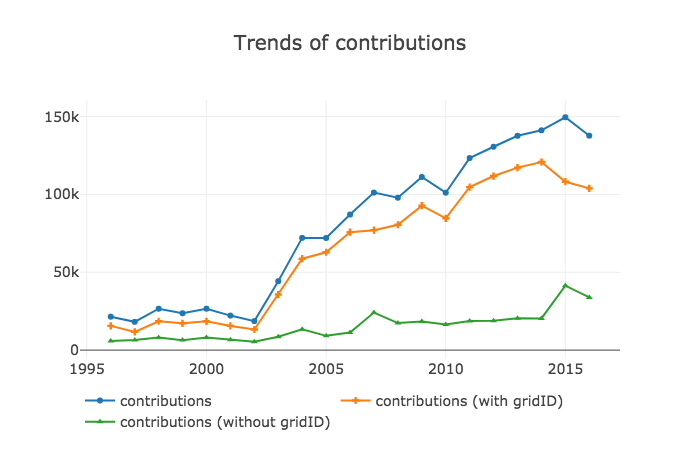
\includegraphics[width=\textwidth]{images/macro_contributions.png}
	\caption[ ]{}
	\label{fig:macro_contributions}
\end{subfigure}%
\begin{subfigure}{.5\textwidth}
	\centering
	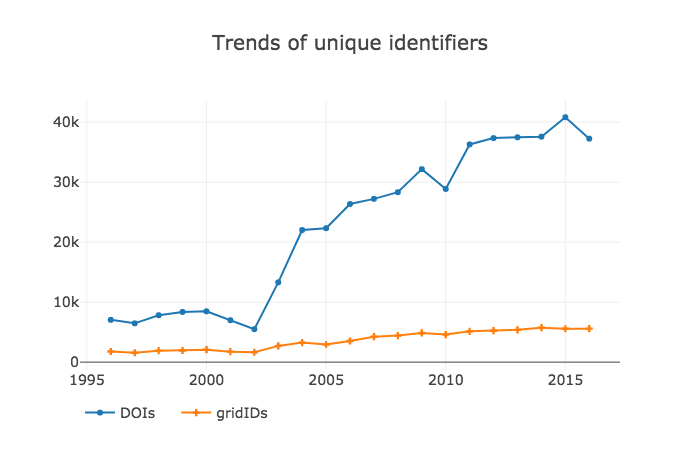
\includegraphics[width=\textwidth]{images/macro_identifiers.png}
	\caption[ ]{}
	\label{fig:macro_identifiers}
\end{subfigure}
\caption{Trends of contributions (with and without resolved affiliations), papers and institutions}
\label{fig:macro_preliminary}
\end{figure}

%Accordingly to our hypothesis about authors' roles in papers,
Figure~\ref{fig:macro_gridids_vs_authors} presents the number of institutions involved in research over time and highlights in two dedicated series the number of institutions appearing as affiliations of the first (in yellow) and last authors (in green) respectively. 
For the sake of clarity, we included also the differential trend (in red) between first/last authors' affiliations and all the others, by computing $gridIDs_{total} - mean(gridIDs_{first}, gridIDs_{last})$.
The figure suggests that there is a substantial gap between the number of institutions that initiate (first author) and overseer (last author) a research endeavour versus the total number of institutions involved in research.
Also, this gap appears to grow over time despite the fact that the average number of authors per paper does not exhibit the same growth, oscillating steadily between 2.6 and 3.3 in the same time interval (not reported here for space reasons, but available online). We will investigate this phenomenon further in the micro analysis.
%
\begin{figure}[t]
\begin{subfigure}{.5\textwidth}
    \centering
	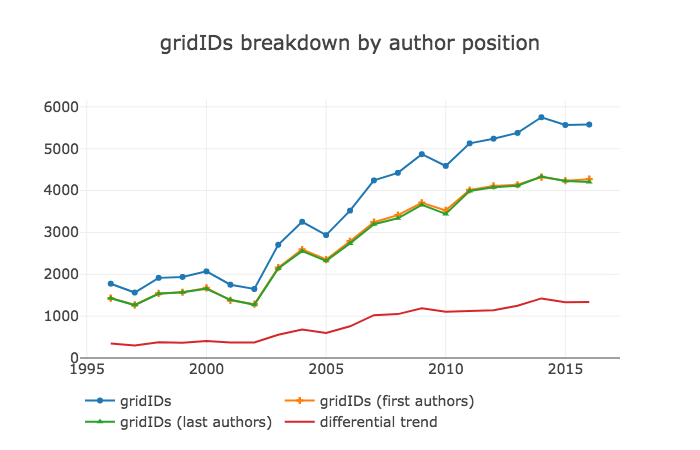
\includegraphics[width=\textwidth]{images/macro_gridids_vs_authors.png}
	\caption[ ]{}
	\label{fig:macro_gridids_vs_authors}
\end{subfigure}%
\begin{subfigure}{.5\textwidth}
	\centering
	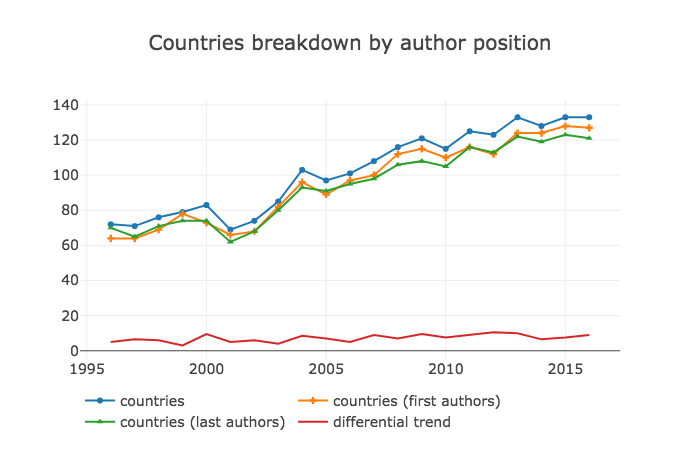
\includegraphics[width=\textwidth]{images/macro_countries_vs_authors.png}
	\caption[ ]{}
	\label{fig:macro_countries_vs_authors}
\end{subfigure}
\caption{Institutions and countries breakdown according to author position}
\label{fig:macro_vs_authors}
\end{figure}
%
\begin{figure}[t]
\begin{subfigure}{.5\textwidth}
	\centering
    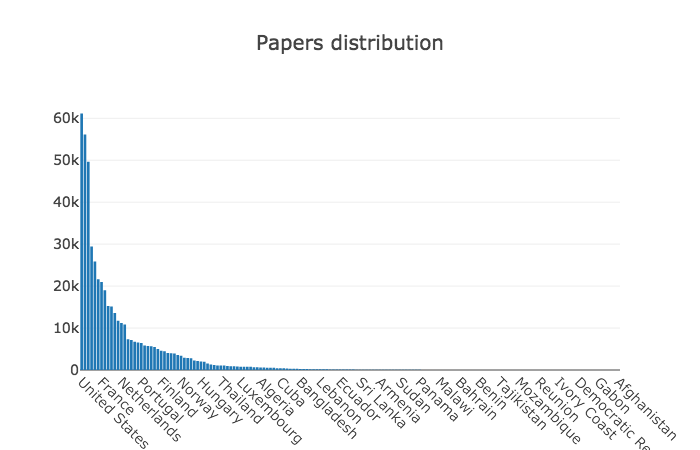
\includegraphics[width=\textwidth]{images/macro_dois_longtail.png}\llap{\raisebox{1cm}{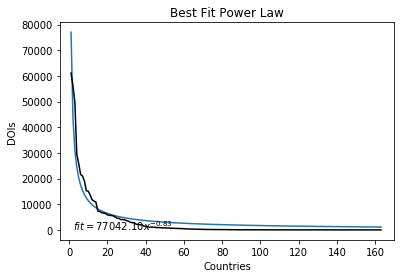
\includegraphics[width=.5\textwidth]{images/macro_dois_powerlaw.png}}}
	\caption[ ]{}
	\label{fig:macro_dois_longtail}
\end{subfigure}%
\begin{subfigure}{.5\textwidth}
	\centering
    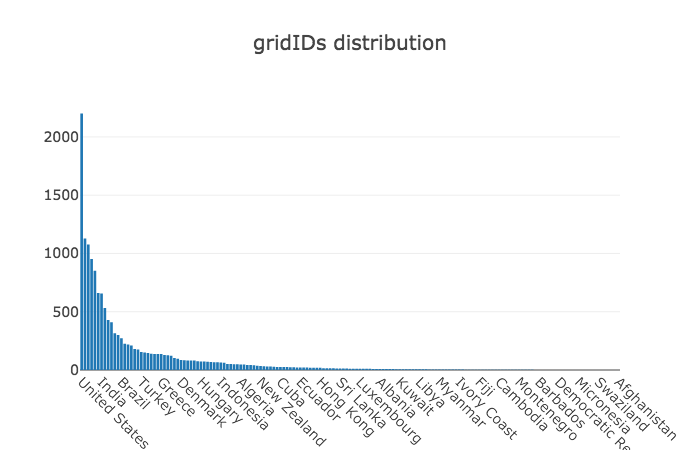
\includegraphics[width=\textwidth]{images/macro_gridids_longtail.png}\llap{\raisebox{1cm}{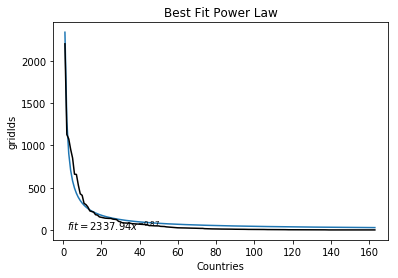
\includegraphics[width=.5\textwidth]{images/macro_gridids_powerlaw.png}}}
	\caption[ ]{}
	\label{fig:macro_gridids_longtail}
\end{subfigure}
\caption{Papers and institutions distributions across countries and their power law approximation}
\label{fig:macro_longtail}
\end{figure}

Similarly, Figure~\ref{fig:macro_countries_vs_authors} highlights the trend of countries in function of author position.
Also in this case, we see a gap between the number of first/last authors' countries of affiliation and the total number of countries involved in research.
The differential trend oscillate from 5 to 9 over the observed period, despite being not remarkably growing as in the case of institutions.
We believe that this is due to the naturally limited number of countries, as opposed to the virtually unbounded number of new institutions that keep appearing each year.

Figure~\ref{fig:macro_dois_longtail} reports the distribution of papers among countries over the observed period without taking initiators and overseers into account.
The distribution is heavily skewed in favour of USA, China, and Germany, highlighting a potential bias in the dataset.
Indeed, a manual inspection of the dataset revealed the presence of many local Asian, Chinese, German, and American conferences.
Despite the potential bias, the power law characteristic of the distribution is evident. In the figure inset, we report the best fit power law obtained by fitting the data points with the least squares method to a power law function of the type $y = ax^s$, with $s<0$.
Interestingly, the power law characteristic of the paper distribution over countries is also valid in each year across the period. 
We verified this by checking Pareto rule\cite{pareto1971translation} for every year, and discovered that invariably 20\% of the countries produces more than 80\% of the papers.

The distribution of institutions over countries (i.e. the number of institutions present in a given country) follows as well a power law, as shown by Figure~\ref{fig:macro_gridids_longtail}.
For the sake of space, we omitted the details about the distributions of papers for first and last authors, which the reader can consult online.

We also noticed that the average $r_{change}$ for the top-5, top-10 and top-25 across the observed period yielded 0.13, 0.09, and 0.08 respectively. This suggests that 
\begin{enumerate*}[label=(\roman*)]
\item year by year it is fairly hard for outsiders to break in a top-$n$, and 
\item that it gets harder and harder as the top-$n$ set broadens.
\end{enumerate*}
In addition, over the 21 year span of our observation, the top-5 has been visited by 10 countries, the top-10 by 16 and the top-25 by 36. 
For example, the top-10 has been visited by USA (21), Germany (21), Japan (21), United Kingdom (21), Italy (21), France (21), Spain (19), Canada (16), China(13), Netherlands (9), South Korea (6), India (6), Poland (5), Russia (4), Australia (3), Switzerland (3); further details are available  online.




\subsection{Micro analysis}
Here we summarise the results obtained by analysing the three high-tier conferences (i.e., ISWC, ESWC and TPDL).

%Here we summarise the results obtained in the micro analysis and we present the results about the selected conferences (i.e. ISWC, ESWC and TPDL)

%grouped in order to facilitate their comparison.
% In the micro analysis we focused on three conferences close to our domain of expertise, namely the International Semantic Web Conference (ISWC), the Extended Semantic Web Conference (ESWC) and the International Conference on Theory and Practice of Digital Libraries (TPDL).

Figure~\ref{fig:contributions} and Figure~\ref{fig:identifiers} show respectively the number of contributions, and the number of papers and institutions contributing to the conferences over the years.
Since we manually curated the three datasets, the percentage of unresolved affiliations is much lower than the one of the macro analysis.
Again we can observe a high correlation between the number of papers accepted and the number of contributing institutions.
As opposed to what we observed in the macro analysis, this time the number of papers and institutions are within the same order of magnitude.
This can be explained considering that the number of papers accepted each year by a conference is naturally limited, whereas there is not limitation to the number of institutions that can apply.
%This can be explained considering the conference-focused extent of this analysis; while the organisation committee of a single conferences usually caps the number of maximum paper to accept, there is not virtual limitation for the number of institutions and collaborations that can apply. 
%
\begin{figure}[t]
\begin{subfigure}{.5\textwidth}
	\centering
	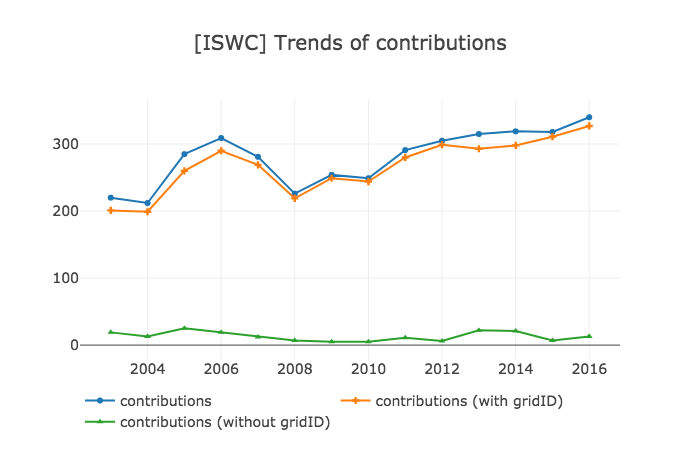
\includegraphics[width=\textwidth]{images/iswc_contributions.png}
	\caption[ ]{}
	\label{fig:iswc_contributions}
\end{subfigure}%
\begin{subfigure}{.5\textwidth}
	\centering
	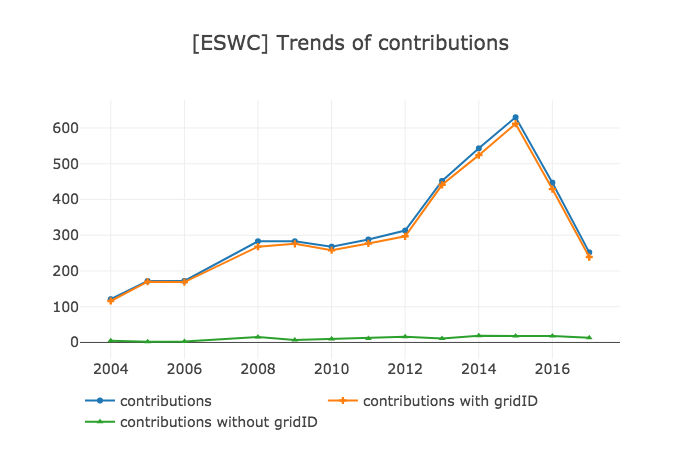
\includegraphics[width=\textwidth]{images/eswc_contributions.png}
	\caption[ ]{}
	\label{fig:eswc_contributions}
\end{subfigure}
	\centering
\begin{subfigure}{.5\textwidth}
	\centering
	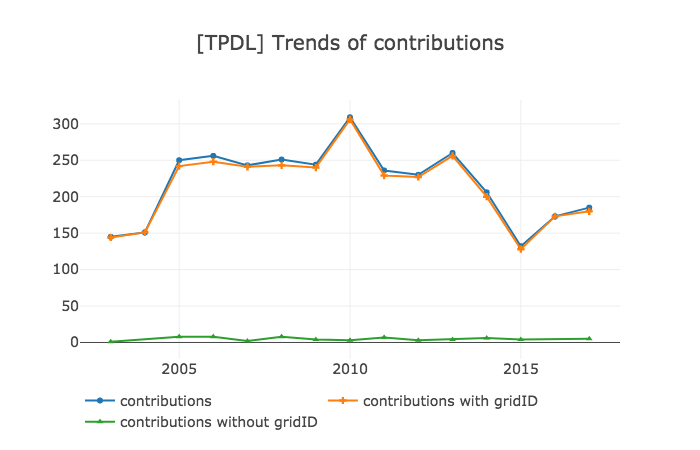
\includegraphics[width=\textwidth]{images/tpdl_contributions.png}
	\caption[ ]{}
	\label{fig:tpdl_contributions}
\end{subfigure}
\caption{Trends of contributions with and without resolved affiliations}
\label{fig:contributions}
\end{figure}
%
\begin{figure}[t]
\begin{subfigure}{.5\textwidth}
	\centering
	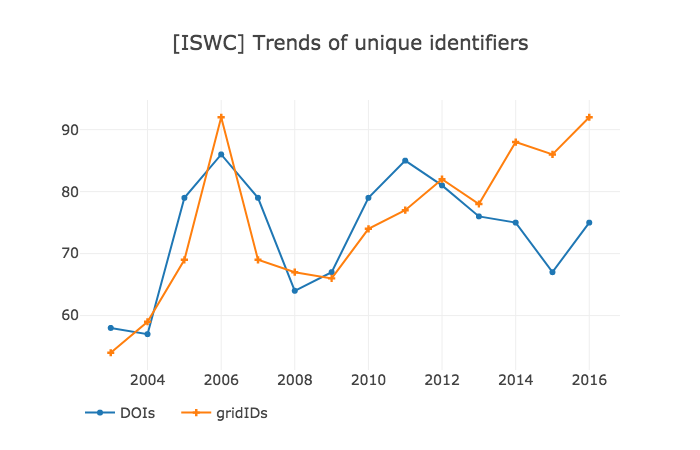
\includegraphics[width=\textwidth]{images/iswc_identifiers.png}
	\caption[ ]{}
	\label{fig:iswc_identifiers}
\end{subfigure}%
\begin{subfigure}{.5\textwidth}
	\centering
	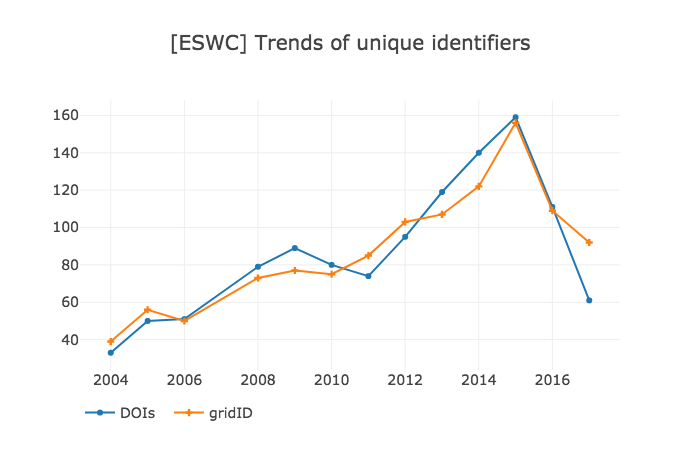
\includegraphics[width=\textwidth]{images/eswc_identifiers.png}
	\caption[ ]{}
	\label{fig:eswc_identifiers}
\end{subfigure}
	\centering
\begin{subfigure}{.5\textwidth}
	\centering
	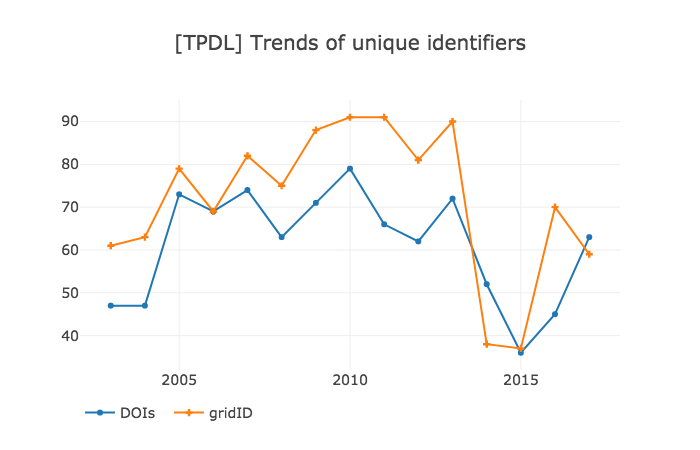
\includegraphics[width=\textwidth]{images/tpdl_identifiers.png}
	\caption[ ]{}
	\label{fig:tpdl_identifiers}
\end{subfigure}
\caption{Trends of papers and institutions}
\label{fig:identifiers}
\end{figure}

Similar to what was observed in the macro analysis, Figure~\ref{fig:gridids_vs_authors} shows the number of institutions contributing to the conferences and highlights the trends of the ones appearing as first and last authors' affiliations. 
As in the previous analysis, the growing gap between the institutions associated with first/last authors and the total number of affiliations is present for all the three conferences as suggested by the differential trend.

We investigated further and retrieved the sets of institutions never appearing as either first or last authors' affiliations throughout the entire observed periods (available online). 
Here it can be noted how prestigious universities and research centres appear side by side with smaller firms and less well-known universities or institutions.
This result indicates that the gap is ``populated'' by institutions that at some point collaborated in semantic web research (or digital libraries) making it through, whereas they never stand out on their own (for reasons beyond our knowledge) in the communities of the respective conferences.
Institutions like national libraries, the European Bioinformatics Institute, the British Geological Survey, the National Institute of Standards and Technology, and so on, provided interesting research case studies or support that eventually culminated in a publication, but apparently never happened to author a paper on their own.
We also verified that the intersection between these sets across different conferences is not empty, suggesting that a few institutions struggled to surface as key contributors, despite being present in either community.

It is important to stress that the sets of institutions appearing as first/last authors' affiliation in different years are very likely to differ; it is not the intention of this study to suggest that institutions initiating or overseeing research are essentially unaltered throughout time.
%
\begin{figure}[t]
\begin{subfigure}{.5\textwidth}
	\centering
	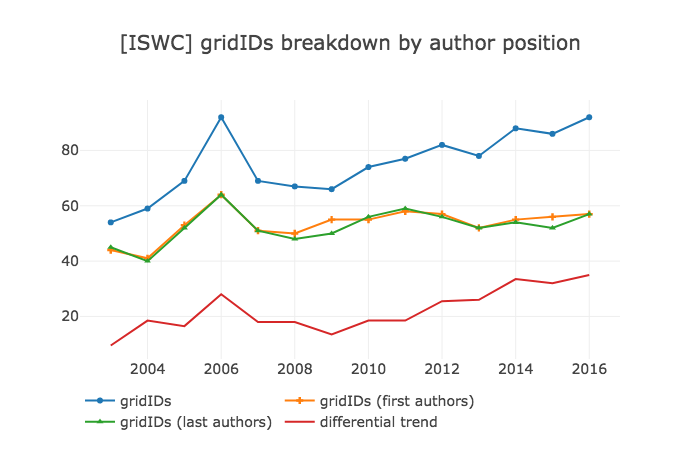
\includegraphics[width=\textwidth]{images/iswc_gridids_vs_authors.png}
	\caption[ ]{}
	\label{fig:iswc_gridids_vs_authors}
\end{subfigure}%
\begin{subfigure}{.5\textwidth}
	\centering
	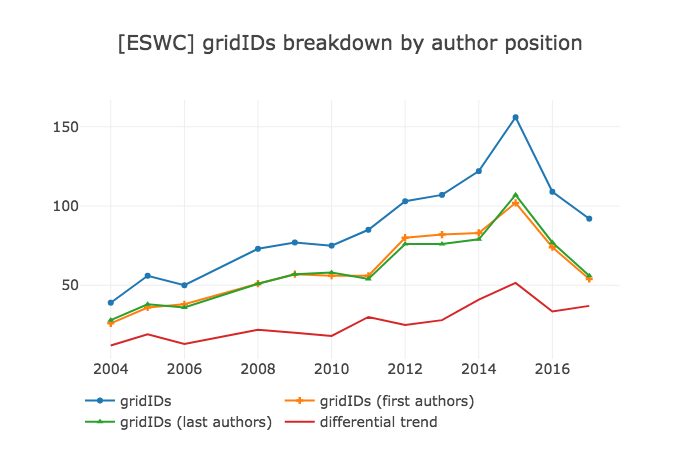
\includegraphics[width=\textwidth]{images/eswc_gridids_vs_authors.png}
	\caption[ ]{}
	\label{fig:eswc_gridids_vs_authors}
\end{subfigure}
\centering
\begin{subfigure}{.5\textwidth}
	\centering
	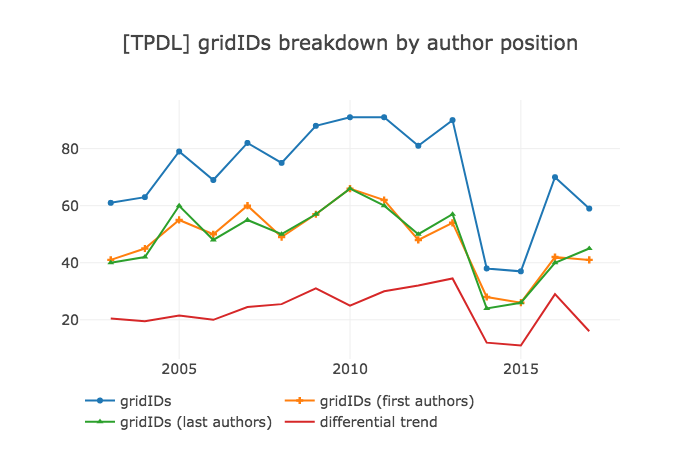
\includegraphics[width=\textwidth]{images/tpdl_gridids_vs_authors.png}
	\caption[ ]{}
	\label{fig:tpdl_gridids_vs_authors}
\end{subfigure}
\caption{Institutions breakdown according to author position}
\label{fig:gridids_vs_authors}
\end{figure}

Figure~\ref{fig:countries_vs_authors} shows the trend of countries contributing to the conferences, highlighting country affiliations of first and last authors.
Consistently to what we observed in the macro analysis a gap is present and growing.
%
\begin{figure}[t]
\begin{subfigure}{.5\textwidth}
	\centering
	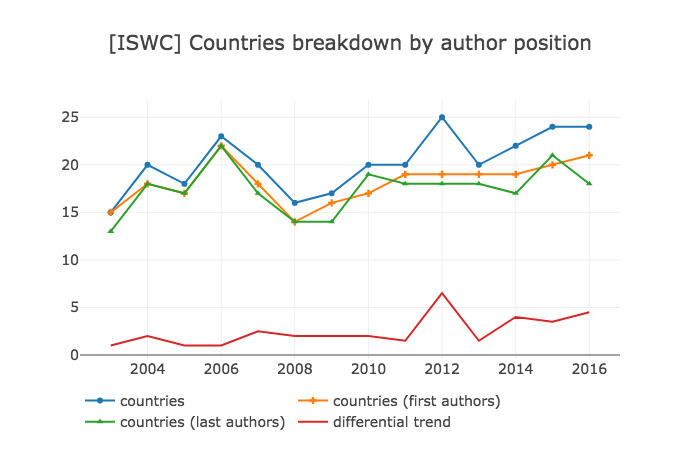
\includegraphics[width=\textwidth]{images/iswc_countries_vs_authors.png}
	\caption[ ]{}
	\label{fig:iswc_countries_vs_authors}
\end{subfigure}%
\begin{subfigure}{.5\textwidth}
	\centering
	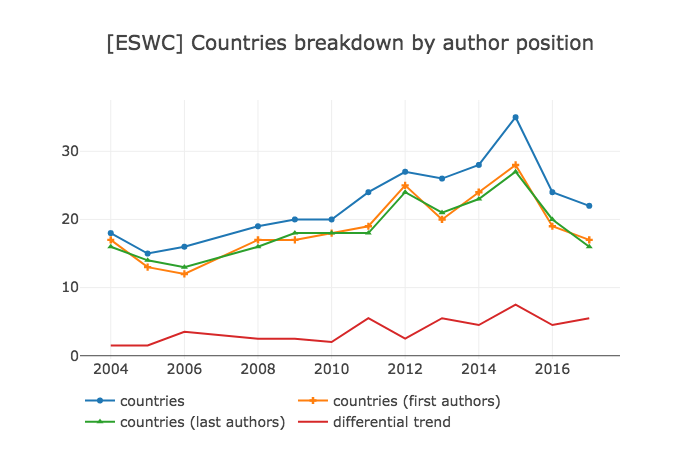
\includegraphics[width=\textwidth]{images/eswc_countries_vs_authors.png}
	\caption[ ]{}
	\label{fig:eswc_countries_vs_authors}
\end{subfigure}
\centering
\begin{subfigure}{.5\textwidth}
	\centering
	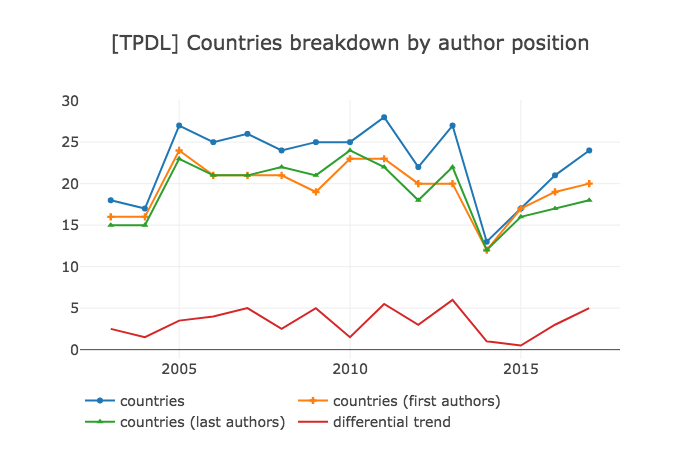
\includegraphics[width=\textwidth]{images/tpdl_countries_vs_authors.png}
	\caption[ ]{}
	\label{fig:tpdl_countries_vs_authors}
\end{subfigure}
\caption{Countries breakdown according to author position}
\label{fig:countries_vs_authors}
\end{figure}

Figure~\ref{fig:dois_longtail} and Figure~\ref{fig:gridids_longtail} again confirm the results shown in previous section even at micro level: the distribution of papers and institutions across countries indeed follows a power law.
However, the power law characteristic surfaces only across the entire observed period as, in general, in a single year the Pareto rule might not be verified mainly because of insufficient data points (i.e. in a single conference edition the number of papers is limited).
In this case, evaluating a top-$n$ stratified rate of change for single conferences gets difficult as the set of countries participating in a single year can be quite limited.
However, as can be seen in the results online, the situation in the top-10 achieves an average $r_{change} \approx 0.23$.
Moreover, it appears that the top-10 is regularly visited by a small number of countries. 
In particular, in ISWC only 13 countries enter the top-10 more then 3 times in the 14 year period.
Similarly, only 14 countries enter the top-10 in ESWC and TPDL. 

Finally, we noticed a stronger presence of European countries in ESWC than in the other two conferences; this is probably due to the initial local target of the conference.
China is quite involved in the semantic web community, but, perhaps surprising, is less active in the TPDL conference and never appears in the top-10.
%
\begin{figure}[t]
\begin{subfigure}{.5\textwidth}
	\centering
    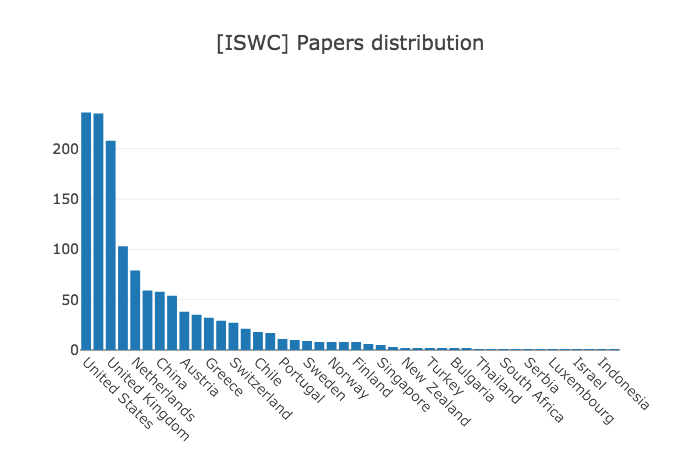
\includegraphics[width=\textwidth]{images/iswc_dois_longtail.png}\llap{\raisebox{1cm}{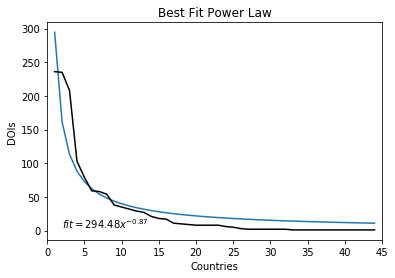
\includegraphics[width=.5\textwidth]{images/iswc_dois_powerlaw.png}}}
	\caption[ ]{}
	\label{fig:iswc_dois_longtail}
\end{subfigure}%
\begin{subfigure}{.5\textwidth}
	\centering
    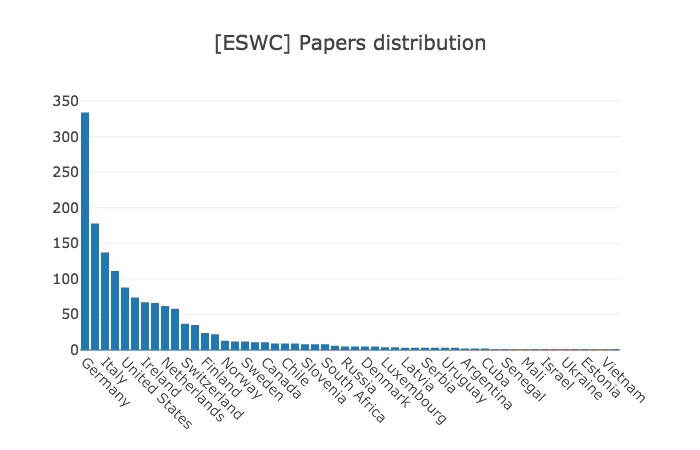
\includegraphics[width=\textwidth]{images/eswc_dois_longtail.png}\llap{\raisebox{1cm}{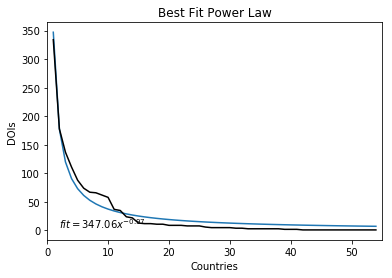
\includegraphics[width=.5\textwidth]{images/eswc_dois_powerlaw.png}}}
	\caption[ ]{}
	\label{fig:eswc_dois_longtail}
\end{subfigure}
\centering
\begin{subfigure}{.5\textwidth}
	\centering
    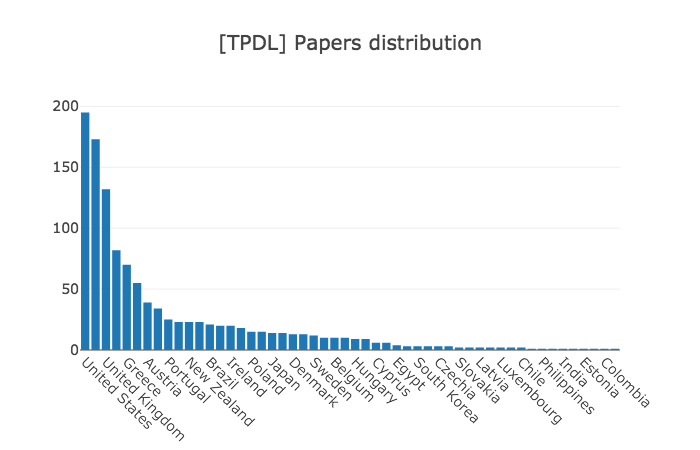
\includegraphics[width=\textwidth]{images/tpdl_dois_longtail.png}\llap{\raisebox{1cm}{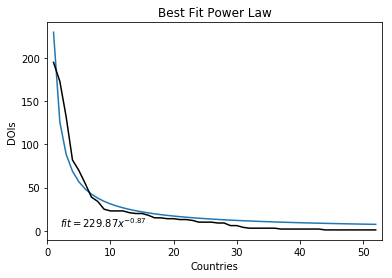
\includegraphics[width=.5\textwidth]{images/tpdl_dois_powerlaw.png}}}
	\caption[ ]{}
	\label{fig:tpdl_dois_longtail}
\end{subfigure}
\caption{Paper distributions across countries and power law approximations}
\label{fig:dois_longtail}
\end{figure}
%
\begin{figure}[h]
\begin{subfigure}{.5\textwidth}
	\centering
    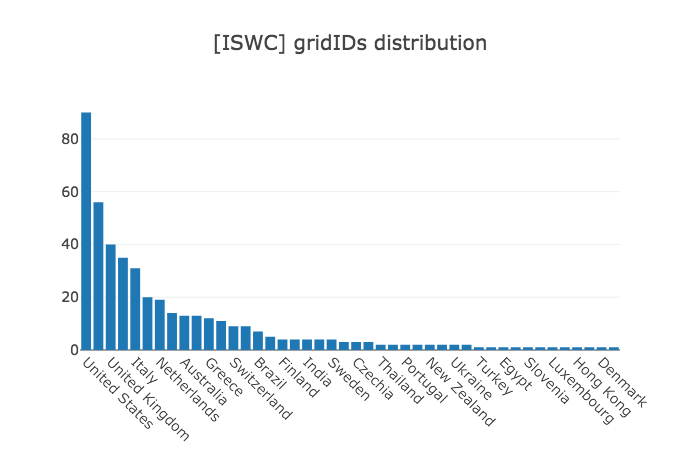
\includegraphics[width=\textwidth]{images/iswc_gridids_longtail.png}\llap{\raisebox{1cm}{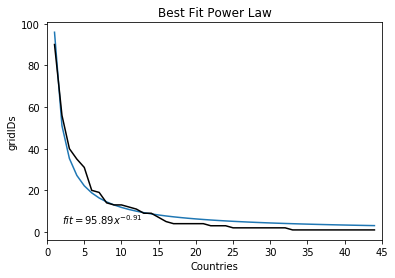
\includegraphics[width=.5\textwidth]{images/iswc_gridids_powerlaw.png}}}
	\caption[ ]{}
	\label{fig:iswc_gridids_longtail}
\end{subfigure}%
\begin{subfigure}{.5\textwidth}
	\centering
    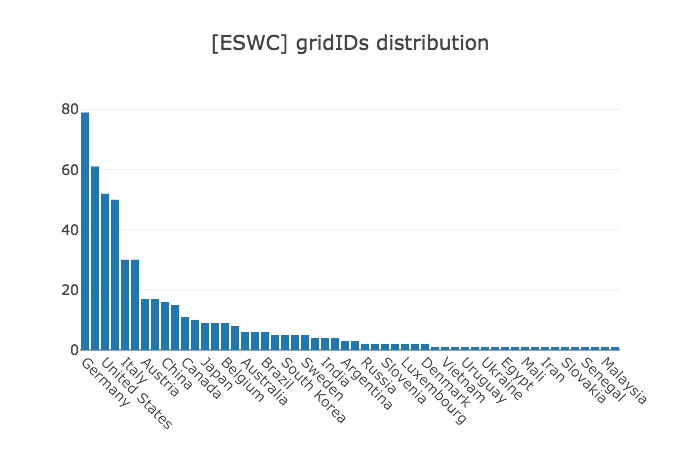
\includegraphics[width=\textwidth]{images/eswc_gridids_longtail.png}\llap{\raisebox{1cm}{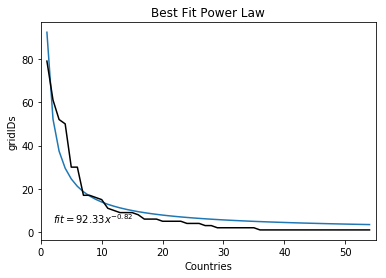
\includegraphics[width=.5\textwidth]{images/eswc_gridids_powerlaw.png}}}
	\caption[ ]{}
	\label{fig:eswc_gridids_longtail}
\end{subfigure}
\centering
\begin{subfigure}{.5\textwidth}
	\centering
    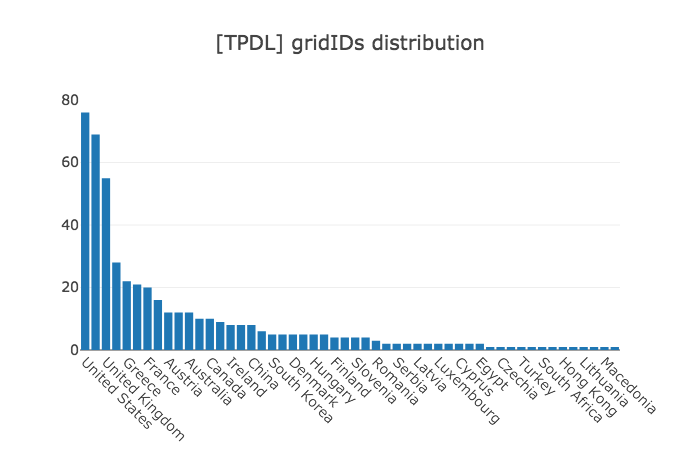
\includegraphics[width=\textwidth]{images/tpdl_gridids_longtail.png}\llap{\raisebox{1cm}{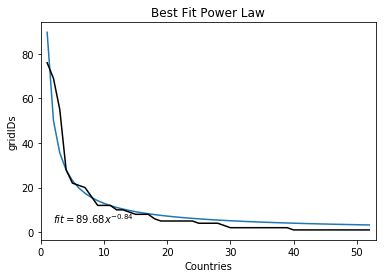
\includegraphics[width=.5\textwidth]{images/tpdl_gridids_powerlaw.png}}}
	\caption[ ]{}
	\label{fig:tpdl_gridids_longtail}
\end{subfigure}
\caption{gridIDs distributions across countries and power law approximations}
\label{fig:gridids_longtail}
\end{figure}


\section{Discussion}
\label{sec:discussion}
The study of authors' affiliations in research literature has been performed for decades as it can provide answers to socioeconomic questions and frame academic research on a geopolitical canvas rather than studying it as an isolated complex system.
In this work we analysed four datasets distilled from Springer Nature Scigraph and provided results on both a macro and a micro scale, focusing on three different high-tier conferences.

The results, in accordance with previous studies~\cite{may1997,king2004a,pan2012}, showed that distributions of papers and institutions across countries still exhibit a power law characteristic in the period 1996-2016.
In addition, our analysis of the turnover rate highlights that not only top ranks in research are limited to a handful of countries and institutions, but that the situation appears also to be stagnant towards the lower ranks.
In general, this reflects the intuition that well-formed research communities exhibit a sort of resistance towards the permeation of outsiders not always sharing knowledge and best practices consolidated over the years.
Therefore, we believe that this phenomenon is worth studying further.
Besides, the papers eventually accepted in conferences is a minimal fraction of the whole amount of submissions; a much clearer view about openness/closeness of conferences and research communities could be achieved by having access to data about rejected papers held in conference management systems such as EasyChair\footnote{EasyChair conference management system, \url{http://easychair.org}} or ConfTool\footnote{ConfTool conference \& event management software, \url{http://www.conftool.net}}.

The results from our study on first and last authors' affiliations show that, in principle, weighting authors' contributions is an intuition that can provide different keys to interpret data. 
Other studies dealing with researchers' seniority, for example, take into account the volume of publications produced by a single author throughout a sliding window of $W$ years~\cite{Verleysen2016}, or the number of consecutive years of publishing activity~\cite{Jadidi2017}.
We intend to further investigate these techniques and test further our intuition in order to understand its applicability in other disciplines and extend the approach by including other metrics (e.g., seniority); nonetheless, the preliminary results are indeed interesting.

Furthermore, a final remark has to be spent about the very peculiar nature of the data here considered: conference papers; usually not covered by traditional scientometrics and bibliometrics studies that instead mainly focus on journals.
Unlike journal papers, having a publication accepted in conference proceedings often requires that at least an author is registered to the event and presents the work at the venue.
This aspect has major implications that need to be studied further.
For example, scientists' mobility is subject to economic and geopolitical factors such as geographic distance, budget availability for travels, and travel bans.
In some cases, being physically present at the conference venue means taking long-haul flights; for some countries, such as Australia and similarly rather isolated countries, the chances of being poorly connected to the conference venues are high.
In other cases, despite feasible connections are available, the physical attendance might be hindered by economic factors, that in turn can depend on strategic and political decisions within the single country.
Finally, factors driven by international politics can play a major role too.
In several occasions, travel bans disrupted scientists' mobility; in 2013, for example, NASA prevented Chinese nationals to set foot in the space agency's Ames research centre in California\footnote{\url{https://www.theguardian.com/science/2013/oct/05/us-scientists-boycott-nasa-china-ban}}.
Furthermore, citizens of countries with an important Muslim background always have encountered more difficulties for getting travel visas to European or USA countries. 
In addition, recent USA's international policies and travel restrictions, possibly have made this even worse~\cite{morello2017scientists}.
However, it has to be noted that these concerns about researchers' freedom of movement affect only conference papers in which all the authors are subject to the same kind of restrictions; in the case of papers whose authors have heterogeneous affiliations, for example, the author with less restrictive constraints is, in principle, free to reach the venue and present the findings on behalf of the colleagues.
All these implications are worth studying.
To this end, a future extension of this work could include the comparison of country rankings among high-tier conferences and journals from a controlled set of academic fields in order to analyse whether the freedom of mobility has an impact or not on how countries perform.

In conclusion, we advocate openness and transparency for research literature metadata. It is detrimental to research itself to relinquish information about venues, papers, authorship and much more in data silos hard (or almost impossible) to access.
Datasets like SciGraph are a bless for researchers working on scholarly analytics and such initiatives should be fostered.
Moreover, new best practices for declaring unambiguous authors' affiliations should be devised in order to facilitate the work of researcher working with scholarly knowledge.
Being able to access high quality research literature metadata is key for enabling large-scale analytics and cross-correlate scholarly knowledge with external datasets and hopefully get better and more thorough insight on the existing global dynamics prevailing in academic research.


\section*{Acknowledgements}
We would like to thank the SciGraph team, especially Dr. Michele Pasin, whose work and prompt response made this study possible.


%
% ---- Bibliography ----
\bibliographystyle{splncs03}
\bibliography{biblio}

\end{document}